\Chapter{Methodology}

Your methodology tends to fit in well immediately after your literature review, and should flow from it, e.g. the methodology pulling on thing in the lit review.

At this (methodology) point you should have already defined your research question (in the intro) and conducted a review of what other scholars have done on the topic, as part of the lit review (but note, as per the guidelines provided for the lit review, that chapter isn't all about what others have done in the focus you chose but may include other things like important theories and technologies that you are building on). 

In planning your methodology, you will likely use insights from the articles and books you read in your literature review -- together with advice from your supervisor and other project stakeholders -- to decide how you will address your research objective (or research question or hypothesis) that you set in Chapter 1. These plans for an engineering project are likely about how you will choose components and tools (both software and hardware tools), what to prototype and how to build the prototype, how to gather data, how do testing, etc. Remember that you need to show some logical reasoning for why you chose the methods and approach you are using (possibly referring back to supportive items of lit review or even meeting minutes, which can also be referenced).

The methodology is probably the piece that will be the most critically interrogated by your examiners -- because it is demonstrating your understanding of the research process and also a deep understanding of your discipline and your ability to choose effective practices.  Thus, to emphasise what the methodology is: it is describing the methods you followed in your research project for the development and experimentation of a solution to solve (or mitigate) a problem together with how testing was carried out to show how that problem was solved or reduced using your approach. \textbf{\textit{Note}} that not all engineering projects are a build and test undertaking; please ensure to choose an appropriate methodology and writing structure for your specific project and to do so in collaboration with your supervisor. \footnote{Note that, yes, unfortunately it is sometimes not possible to provide an effective solution to the chosen problem -- it may be too expensive or take too long to solve properly -- but even then it can still be considered a contribution of knowledge and still have some value as a research investigation.}

\textbf{Methodology vs Design:} A vitally important terminology consideration is to realize that  methodology is not the same as design. This is a common confusion amongst students who have not done a research project or written a thesis before. This short explanation should suffice to ensure you understand the difference:

\begin{itemize}
	\item Methodology: this describes how you are going to go about doing the research project. It describes the main high-level steps (or phases) of the project. It does not detail design or pieces of your design. You should not need any block diagrams in the design.
	\item Design: this is what you have built (or are going to build). It includes diagrams, system block diagram, flow charts, pseudocode/algorithms, schematics, etc. Generally, in a computing-related project, it will end off with implementation details (actual code snippets). These implementation details, depending on how much there are of them, may be better placed in a separate Implementation chapter. Similarly, you might decide to have a separate Integration chapter if there are a lot of pieces that takes quite a bit of explaining and diagrams to describe how they connect and work together. 
\end{itemize}

\textbf{\color{red}Brief points about methodology structure}
\begin{itemize}
	\item The start of your methodology should give a brief outline of what is involved (just a paragraph or two). 
	\item Part of the intro blurb to this chapter should also indicate how you build upon some literature; some considerations of how your methodology was inspired/influenced by other work that you have read.
	\item Typically an easy and clear approach is presenting your methodology as a series of phases i.e. a bit inspired by the Waterfall Model (Royce, 1970). While the Waterfall Model may suggest the big pieces, Boehm's Spiral Model may be more the reality of how the project was carried out (i.e. in an interactive process in which progress and potential risks were assessed and reassessed at various stages during the project.)
	\item Do not cover the details of the specific design, that is for the design chapter. But do cover the stages surrounding the design as well as the big pieces of the design activities.
	\item Explain your experiment approach, important/specialized metrics used, etc.
\end{itemize}


\section{Suggested Structure}

\begin{itemize}
	\item Overview of Approach / Plan of action (possibly including an overview or flow diagram showing a visualization of the methodology process)
	\item Answering the 'How it is done question' (possibly including discussion of metrics used)
	\item Phases of the research project, or Steps taken to perform the research
	\item Experiment design (experimental design \textit{is not} prototype design, it is the design of experiments to test your prototype or system that you build.)
	\item Data collection methods
	\item Data analysis and interpretation methods
\end{itemize}

Please see Figure \ref{methododviz} for illustration on the structuring of a research methodology. There may be some back-and-forth at least in the initial stage of the project in deciding the objectives or research questions to choose for the study, you may or may not decide to start you methodology description from such a point (i.e. you might want to rather start with discussing the initial lit review in the understanding that there was a prior process in deciding the actual focus for the study which you and your supervisor may decide is out of the scope for the writeup.)

\begin{figure}
	\centering
	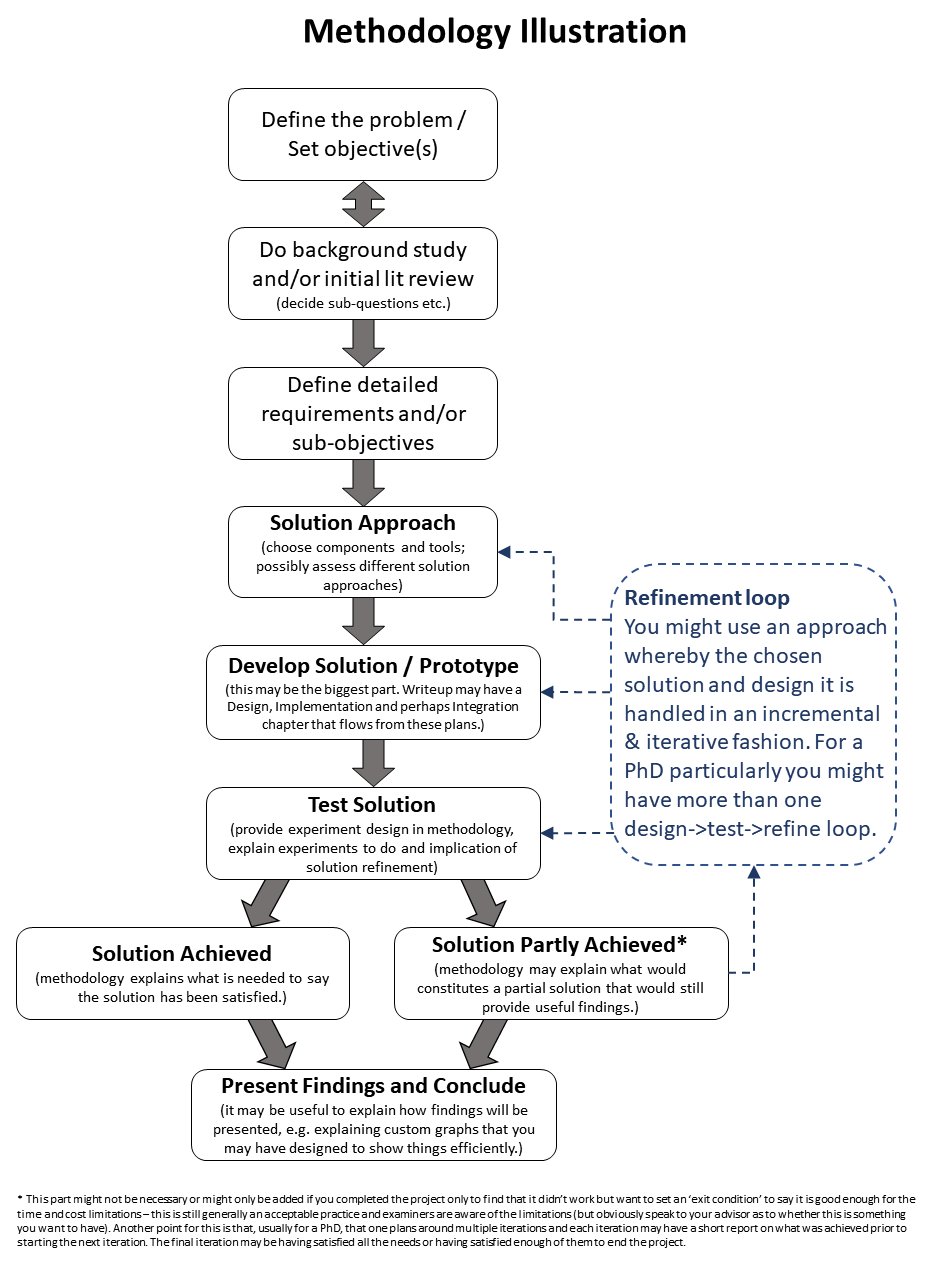
\includegraphics[width=0.9\linewidth]{Chapters/Figures/methodology.png}
	\caption{Example methodology structure and example of how to visualize your methodology}
	\label{fig:methododviz}
\end{figure}

\emph{Thoughts on using an Appendix}: You want to keep your methodology chapter focussed and easy-to-read (but obviously not simplistic). An appendix to the methodology can help keep it focused and uncluttered. For material that is useful in supporting or explaining your method, but is perhaps a bit indirectly connected or at a rather low-level that distracts from explaining the overall method clearly, you could put such details in an appendix (e.g. as supporting material that might clarify, at a lower level, the 'how' and 'why' aspects of you approach). Appendix items for a methodology typically include: copies of questionnaires, detailed interview questions or plans, interview or meeting schedules, minutes from meetings or correspondence (that you are permitted to make public and feel would support decisions in your project), design sketches, mind-maps or concept drawings.
